\subsection{Obecná rovnice přímky}
\label{subsec:General_line_equation}

V předchozí části jsme přímku popisovali pomocí jednoho jejího bodu,
směrového vektoru a parametru. Změnou parametru jsme postupně získávali
jednotlivé body přímky. Parametrické vyjádření nám tedy říká,
\emph{jak body přímky vytvářet}.

Přímku však můžeme popsat také jiným způsobem: jedinou rovnicí o dvou
proměnných $x$ a $y$, kterou splňují právě souřadnice bodů ležících na
přímce. Taková rovnice nám neříká, jak se po přímce pohybovat, ale
umožňuje snadno rozhodnout, zda daný bod na přímce leží. Tento způsob
popisu nazýváme \textbf{obecnou rovnicí přímky}.

Základní roli při jejím odvození bude hrát vektor kolmý k přímce.

\subsubsection{Normálový vektor přímky}
\label{subsubsec:Normal_vector_line}

Při parametrickém vyjádření jsme směr přímky určovali pomocí směrového
vektoru, který je s přímkou rovnoběžný. Nyní budeme pracovat také
s vektorem, který je ke směru přímky kolmý.

\begin{definition}\label{def:Normal_vector_line}
    \textbf{Normálovým vektorem přímky} $p$ nazýváme každý nenulový
    vektor $\vec{n}$, který je kolmý ke směrovému vektoru této přímky,
    a tedy také k přímce samotné.
\end{definition}

Je-li $\vec{u}$ směrovým vektorem přímky $p$ a $\vec{n}$ jejím
normálovým vektorem, platí
\begin{equation}\label{eq:Direction_normal_dot_product}
    \vec{u}\cdot\vec{n}=0.
\end{equation}

Má-li směrový vektor souřadnice
\[
    \vec{u}=(u_x;u_y),
\]
můžeme podle definice~\ref{def:Fast_orthogonal_vector} zvolit například
normálový vektor
\[
    \vec{n}=(u_y;-u_x)
\]
nebo opačně orientovaný vektor
\[
    \vec{n}=(-u_y;u_x).
\]

Naopak známe-li normálový vektor
\[
    \vec{n}=(a;b),
\]
můžeme jako směrový vektor přímky zvolit například
\begin{equation}\label{eq:Direction_vector_from_normal_vector}
    \vec{u}=(-b;a)
\end{equation}
nebo opačně orientovaný vektor
\[
    \vec{u}=(b;-a).
\]
Skutečně platí
\[
    (a;b)\cdot(-b;a)=-ab+ab=0.
\]

Stejně jako směrový vektor ani normálový vektor není určen jednoznačně.
Je-li $\vec{n}$ normálovým vektorem přímky, potom je jejím normálovým
vektorem také každý jeho nenulový reálný násobek
\[
    k\vec{n},
    \qquad
    k\in\mathbb{R}\setminus\{0\}.
\]
Všechny tyto vektory jsou navzájem rovnoběžné a jsou kolmé k téže
přímce.

\begin{figure}[H]
    \centering
    \begin{tikzpicture}[scale=1]

        \coordinate (A) at (0,0);
        \coordinate (U) at (3,1.5);
        \coordinate (N) at (-0.75,1.5);

        % Přímka
        \draw[thin] (-2,-1) -- (5,2.5) node[right] {$p$};

        % Bod
        \fill (A) circle (2pt) node[below right] {$A$};

        % Směrový a normálový vektor
        \draw[vector] (A) -- (U)
            node[midway, above, sloped] {$\vec{u}$};
        \draw[vector] (A) -- (N)
            node[midway, left] {$\vec{n}$};

        % Pravý úhel
        \draw
            (0.30,0.15)
            --
            (0.15,0.45)
            --
            (-0.15,0.30);

    \end{tikzpicture}
    \caption{Směrový vektor $\vec{u}$ je rovnoběžný s přímkou $p$,
    zatímco normálový vektor $\vec{n}$ je k přímce kolmý.}
    \label{fig:Normal_vector_line}
\end{figure}

\subsubsection{Odvození obecné rovnice přímky}
\label{subsubsec:Derivation_general_line_equation}

Uvažujme přímku $p$, která prochází bodem
\[
    A[x_A;y_A]
\]
a má normálový vektor
\[
    \vec{n}=(a;b),
\]
kde alespoň jedna ze souřadnic $a$, $b$ je nenulová. Dále zvolme
libovolný bod roviny
\[
    X[x;y].
\]

Vektor směřující z bodu $A$ do bodu $X$ má souřadnice
\[
    \overrightarrow{AX}=(x-x_A;y-y_A).
\]

Bod $X$ leží na přímce $p$ právě tehdy, když je vektor
$\overrightarrow{AX}$ rovnoběžný s přímkou. Proto musí být kolmý
k jejímu normálovému vektoru $\vec{n}$. Pomocí skalárního součinu tuto
podmínku zapíšeme jako
\begin{equation}\label{eq:Point_normal_condition_line}
    \vec{n}\cdot\overrightarrow{AX}=0.
\end{equation}

Po dosazení souřadnic obou vektorů dostáváme
\begin{align*}
    (a;b)\cdot(x-x_A;y-y_A)&=0,\\
    a(x-x_A)+b(y-y_A)&=0.
\end{align*}

Rovnice
\begin{equation}\label{eq:Point_normal_line_equation}
    a(x-x_A)+b(y-y_A)=0
\end{equation}
popisuje přímku, která prochází bodem $A[x_A;y_A]$ a má normálový
vektor $\vec{n}=(a;b)$.

\begin{figure}[H]
    \centering
    \begin{tikzpicture}[scale=1]

        \coordinate (A) at (0,0);
        \coordinate (X) at (3,1.5);
        \coordinate (Y) at (2.5,2.6);
        \coordinate (N) at (-0.75,1.5);

        % Přímka
        \draw[thin] (-2,-1) -- (5,2.5) node[right] {$p$};

        % Body
        \fill (A) circle (2pt) node[below right] {$A[x_A;y_A]$};
        \fill (X) circle (2pt) node[below right] {$X[x;y]$};
        \fill (Y) circle (2pt) node[above right] {$Y$};

        % Vektory
        \draw[vector] (A) -- (X)
            node[midway, below, sloped] {$\overrightarrow{AX}$};
        \draw[vector] (A) -- (N)
            node[midway, left] {$\vec{n}=(a;b)$};
        \draw[vector, dashed] (A) -- (Y)
            node[midway, above, sloped] {$\overrightarrow{AY}$};

        % Pravý úhel
        \draw
            (0.30,0.15)
            --
            (0.15,0.45)
            --
            (-0.15,0.30);

    \end{tikzpicture}
    \caption{Bod $X$ leží na přímce $p$, protože vektor
    $\overrightarrow{AX}$ je kolmý k normálovému vektoru $\vec{n}$.
    U bodu $Y$, který na přímce neleží, tato kolmost neplatí.}
    \label{fig:General_line_derivation}
\end{figure}

Roznásobením rovnice \eqref{eq:Point_normal_line_equation} získáme
\begin{align*}
    a(x-x_A)+b(y-y_A)&=0,\\
    ax-ax_A+by-by_A&=0,\\
    ax+by-(ax_A+by_A)&=0.
\end{align*}

Bod $A$ i normálový vektor $\vec{n}$ jsou pevně zvolené, a proto je
výraz
\[
    -(ax_A+by_A)
\]
konstantou. Označíme-li tuto konstantu písmenem $c$, dostáváme rovnici
\[
    ax+by+c=0.
\]

\begin{definition}\label{def:General_line_equation}
    \textbf{Obecnou rovnicí přímky} v rovině nazýváme rovnici tvaru
    \begin{equation}\label{eq:General_line_equation}
        ax+by+c=0,
    \end{equation}
    kde
    \[
        a,b,c\in\mathbb{R}
        \qquad\text{a}\qquad
        (a;b)\neq(0;0).
    \]

    Přímka $p$ je množinou všech bodů $X[x;y]$, jejichž souřadnice
    tuto rovnici splňují, tedy
    \[
        X[x;y]\in p
        \quad\Longleftrightarrow\quad
        ax+by+c=0.
    \]
\end{definition}

Podmínka $(a;b)\neq(0;0)$ je nezbytná. Kdyby platilo současně
$a=0$ a $b=0$, rovnice by se zredukovala na vztah
\[
    c=0.
\]
Pro $c=0$ by tuto rovnici splňoval každý bod roviny, zatímco pro
$c\neq0$ by ji nesplňoval žádný bod. Ani v jednom případě by tedy
rovnice nepopisovala přímku.

\begin{remark}\label{rem:Meaning_coefficients_general_line}
    V obecné rovnici $ax + by + c = 0$ jsou čísla $a$, $b$ a $c$ pevnými koeficienty určujícími konkrétní
    přímku. Proměnné $x$ a $y$ představují souřadnice obecného bodu
    roviny.

    Koeficienty $a$ a $b$ současně tvoří souřadnice normálového vektoru
    přímky:
    \begin{equation}\label{eq:Normal_vector_from_general_line}
        \vec{n}=(a;b).
    \end{equation}

    Jako směrový vektor přímky můžeme zvolit například
    \begin{equation}\label{eq:Direction_vector_from_general_line}
        \vec{u}=(-b;a).
    \end{equation}
\end{remark}

\begin{example}\label{exa:Vectors_from_general_line}
    Určete normálový a směrový vektor přímky
    \[
        p: 3x-4y+7=0.
    \]

    Z koeficientů u proměnných $x$ a $y$ přímo získáme normálový
    vektor
    \[
        \vec{n}=(3;-4).
    \]

    Směrový vektor musí být k normálovému vektoru kolmý. 
    Podle definice~\ref{def:Fast_orthogonal_vector} 
    či vztahu \eqref{eq:Direction_vector_from_general_line} můžeme zvolit
    \[
        \vec{u}=(4;3).
    \]

    Kolmost ověříme skalárním součinem:
    \[
        \vec{n}\cdot\vec{u}
        =
        (3;-4)\cdot(4;3)
        =
        12-12
        =
        0.
    \]

    Přímka $p$ má tedy například normálový vektor
    $\vec{n}=(3;-4)$ a směrový vektor $\vec{u}=(4;3)$. Stejně dobře
    bychom mohli zvolit opačný směrový vektor $\vec{u}=(-4;-3)$.
\end{example}

\subsubsection{Nejednoznačnost obecné rovnice}
\label{subsubsec:Nonunique_general_line_equation}

Obecná rovnice přímky, stejně jako její parametrické vyjádření, není
určena jednoznačně. Vynásobením všech členů rovnice stejným nenulovým
číslem se množina jejích řešení nezmění.

Například rovnice
\[
    x-2y+4=0
\]
a
\[
    3x-6y+12=0
\]
popisují tutéž přímku. Druhá rovnice vznikla vynásobením první
rovnice číslem $3$.

Dvě obecné rovnice
\[
    a_1x+b_1y+c_1=0
\]
a
\[
    a_2x+b_2y+c_2=0
\]
určují tutéž přímku právě tehdy, když existuje číslo
$k\in\mathbb{R}\setminus\{0\}$ takové, že
\[
    (a_2;b_2;c_2)=k(a_1;b_1;c_1).
\]

\begin{remark}
    Při zjednodušování obecné rovnice můžeme všechny její koeficienty
    vydělit jejich společným nenulovým dělitelem. Rovnici
    \[
        6x-9y+12=0
    \]
    můžeme například vydělit číslem $3$ a získat jednodušší rovnici
    \[
        2x-3y+4=0.
    \]
    Obě rovnice popisují tutéž přímku.
\end{remark}

\begin{example}\label{exa:Equivalent_general_line_equations}
    Rozhodněte, které z následujících rovnic popisují tutéž přímku:
    \begin{align*}
        p &: 2x-3y+5=0,\\
        q &: -4x+6y-10=0,\\
        r &: 4x-6y+5=0.
    \end{align*}

    Rovnici $q$ můžeme vydělit číslem $-2$ a získáme tak rovnici:
    \[
        -4x+6y-10=0
        \quad\Longrightarrow\quad
        2x-3y+5=0.
    \]
    Rovnice $p$ a $q$ tedy popisují tutéž přímku. Jejich normálové
    vektory jsou proto lineárně závislé a platí
    \begin{align*}
        (2;-3) &= -\frac{1}{2}\cdot(-4;6),\\
        \vec{n}_p &= -\frac{1}{2}\vec{n}_q.
    \end{align*}

    Normálový vektor přímky $r$ je
    \[
        \vec{n}_r=(4;-6)=2\vec{n}_p,
    \]
    takže přímka $r$ má stejný směr jako přímky $p$ a $q$. Trojice
    koeficientů její obecné rovnice však není stejným násobkem trojice
    koeficientů rovnice přímky $p$. Přímka $r$ proto není s přímkami
    $p$ a $q$ totožná, což je patrné také z grafického znázornění
    na obrázku~\ref{fig:Equivalent_general_line_equations}.
    \begin{figure}[H]
        \centering
        \begin{tikzpicture}
            % body
            \coordinate (P_1) at (-4, -1);
            \coordinate (P_2) at (2, 3);
            \coordinate (R_1) at (-2.75, -1);
            \coordinate (R_2) at (3.25, 3);

            % osy x a y
            \draw [<->] (-5,0) -- (5,0) node[right] {$x$};
            \draw [<->] (0,-2) -- (0,4) node[above] {$y$};

            % Jednotky na osách
            \foreach \x in {-4,-3,-2,-1,1,2,3,4} {
                \draw (\x,0.1) -- (\x,-0.1) node[below] {\x};
            }
            \foreach \y in {-1,1,2,3} {
                \draw (0.1,\y) -- (-0.1,\y) node[left] {\y};
            }
            
            % přímky
            \draw[thick, <->] (P_1) -- (P_2) node[above] {$p = q$};
            \draw[thick, <->] (R_1) -- (R_2) node[right] {$r$};
        \end{tikzpicture}
    \caption{Ekvivalentní obecné rovnice přímek.}
    \label{fig:Equivalent_general_line_equations}
    \end{figure}
\end{example}

\subsubsection{Určení obecné rovnice přímky}
\label{subsubsec:Determining_general_line_equation}

Obecná rovnice přímky je určena jejím normálovým vektorem a jedním
bodem, kterým přímka prochází. Podle způsobu zadání proto nejprve
hledáme vhodný normálový vektor a následně použijeme známý bod přímky.

Pro určení obecné rovnice přímky můžeme využít dva základní postupy.
První z nich je založen na dosazování normálového vektoru a bodu do vztahu
\eqref{eq:General_line_equation} a dopočítání konstanty $c$. 
Druhý je založen na dosazování bodu a normálového vektoru do vztahu \eqref{eq:Point_normal_line_equation} a následné úpravě do obecného tvaru.

\begin{example}\label{exa:General_line_from_point_normal}
    Určete obecnou rovnici přímky $p$, která prochází bodem $P[2;-1]$ a má normálový vektor $\vec{n}=(3;2)$.

    Při prvním postupu dosadíme normálový vektor $\vec{n}=(3;2)$ do vztahu
    \eqref{eq:General_line_equation}:
    \begin{align*}
        ax + by + c &= 0,\\
        3x + 2y + c &= 0.
    \end{align*}

    Nyní dopočítáme konstantu $c$ dosazením souřadnic bodu $P[2;-1]$:
    \begin{align*}
        3\cdot2 + 2\cdot(-1) + c &= 0,\\
        6 - 2 + c &= 0,\\
        c &= -4.
    \end{align*}

    Dostáváme obecnou rovnici přímky
    \[
        p: 3x + 2y - 4 = 0.
    \]


    Při druhém postupu dosadíme bod a normálový vektor do vztahu
    \eqref{eq:Point_normal_line_equation}:
    \begin{align*}
        3(x-2)+2(y-(-1))&=0,\\
        3(x-2)+2(y+1)&=0.
    \end{align*}

    Po roznásobení a úpravě dostáváme
    \begin{align*}
        3x-6+2y+2&=0,\\
        3x+2y-4&=0.
    \end{align*}

    Obecná rovnice hledané přímky je tedy
    \[
        p: 3x+2y-4=0.
    \]

    Jak můžeme vidět, obě metody vedou ke stejnému výsledku.
\end{example}

Je-li přímka určena bodem přímky a její směrový vektor, nejprve ke směrovému
vektoru určíme kolmý normálový vektor. Poté postupujeme stejně jako
v předchozím případě.

\begin{example}\label{exa:General_line_from_point_direction}
    Určete obecnou rovnici přímky $q$, která prochází bodem $A[-1;3]$ a má směrový vektor $\vec{u}=(2;-5)$.
    
    K vektoru $\vec{u}=(2;-5)$ zvolíme kolmý normálový vektor
    \[
        \vec{n}=(5;2).
    \]

    Obecnou rovnici přímky nejprve zapíšeme s neurčeným absolutním
    členem $c$:
    \begin{align*}
        ax+by+c &= 0,\\
        5x+2y+c &= 0.
    \end{align*}
    Nyní dopočítáme konstantu $c$ dosazením souřadnic bodu $A[-1;3]$:
    \begin{align*}
        5\cdot(-1) + 2\cdot3 + c &= 0,\\
        -5 + 6 + c &= 0,\\
        c &= -1.
    \end{align*}

    Obecná rovnice hledané přímky je
    \[
        q: 5x+2y-1=0.
    \]
\end{example}

Jsou-li dány dva různé body
\[
    A[x_A;y_A],
    \qquad
    B[x_B;y_B],
\]
je směrovým vektorem přímky vektor
\[
    \overrightarrow{AB}=(x_B-x_A;y_B-y_A).
\]
K němu můžeme zvolit normálový vektor
\[
    \vec{n}=(y_A-y_B;x_B-x_A).
\]
Dosazením bodu $A$ do rovnice určené bodem a normálovým vektorem
získáme
\begin{align*}
    &(y_A-y_B)(x-x_A)+(x_B-x_A)(y-y_A)=0,\\
    &(y_A-y_B)x+(x_B-x_A)y+x_Ay_B-x_By_A=0.
\end{align*}

\begin{example}\label{exa:General_line_from_two_points}
    Určete obecnou rovnici přímky $p_{CD}$, která prochází body
    \[
        C[2;2],
        \qquad
        D[-1;3].
    \]

    Nejprve určíme směrový vektor přímky:
    \[
        \overrightarrow{CD}
        =
        (-1-2;3-2)
        =
        (-3;1).
    \]

    K tomuto vektoru zvolíme kolmý normálový vektor
    \[
        \vec{n}=(1;3).
    \]

    Dosadíme vektor $\vec{n}$ a bod $C[2;2]$ do bodově-normálového tvaru rovnice přímky:
    \begin{align*}
        1(x-2)+3(y-2)&=0,\\
        x-2+3y-6&=0,\\
        x+3y-8&=0.
    \end{align*}
    
    Obecná rovnice přímky $p_{CD}$ je tedy
    \[
        p_{CD}: x+3y-8=0.
    \]

    Výsledek ověříme dosazením druhého bodu $D[-1;3]$:
    \[
        -1+3\cdot3-8=-1+9-8=0.
    \]
\end{example}

\begin{example}\label{exa:Points_on_general_line}
    Rozhodněte, zda body $E[1;2]$ a $F[5;1]$ leží na přímce $p: x+3y-8=0$.

    Pro bod $E[1;2]$ dostáváme
    \[
        1+3\cdot2-8
        =
        -1.
    \]
    Protože výsledek není roven nule, bod $E$ na přímce $p$ tedy neleží.

    Pro bod $F[5;1]$ dostáváme
    \[
        5+3\cdot1-8
        =
        0.
    \]
    Bod $F$ proto na přímce $p$ leží.
\end{example}

\subsubsection{Určování bodů přímky}
\label{subsubsec:Finding_points_general_line}

Obecná rovnice přímky je jedna rovnice o dvou proměnných. Má proto
nekonečně mnoho řešení a každé její řešení představuje jeden bod
přímky. Chceme-li určit konkrétní body, zvolíme vhodnou hodnotu jedné
souřadnice a druhou dopočítáme.

Zvlášť užitečné bývá určit průsečíky přímky se souřadnicovými osami:
\begin{itemize}
    \item bod na ose $x$ má souřadnici $y=0$,
    \item bod na ose $y$ má souřadnici $x=0$.
\end{itemize}

Je-li $a\neq0$, protíná přímka osu $x$ v bodě
\begin{equation}\label{eq:General_line_x_intercept}
    P_x\left[-\frac{c}{a};0\right].
\end{equation}
Je-li $b\neq0$, protíná přímka osu $y$ v bodě
\begin{equation}\label{eq:General_line_y_intercept}
    P_y\left[0;-\frac{c}{b}\right].
\end{equation}

\begin{remark}
    Jestliže $a\neq0$ a $b\neq0$, má přímka
    \[
        ax+by+c=0
    \]
    průsečíky s oběma souřadnicovými osami, a to v bodech
    \[
        P_x\left[-\frac{c}{a};0\right],
        \qquad
        P_y\left[0;-\frac{c}{b}\right].
    \]
\end{remark}

\begin{example}\label{exa:Finding_points_general_line}
    Určete tři body přímky
    \[
        p: 2x+3y-6=0
    \]
    a přímku zakreslete do kartézské soustavy souřadnic.

    Nejprve určíme průsečík s osou $x$. Položíme $y=0$:
    \begin{align*}
        2x+3\cdot0-6&=0,\\
        2x&=6,\\
        x&=3.
    \end{align*}
    Na přímce tedy leží bod
    \[
        A[3;0].
    \]

    Ke stejnému výsledku bychom dospěli také podle vztahu \eqref{eq:General_line_x_intercept}:
    \[
        P_x\left[-\frac{-6}{2};0\right]
        =
        P_x[3;0].
    \]

    Nyní určíme průsečík s osou $y$. Položíme $x=0$:
    \begin{align*}
        2\cdot0+3y-6&=0,\\
        3y&=6,\\
        y&=2.
    \end{align*}
    Na přímce leží také bod
    \[
        B[0;2].
    \]

    Ke stejnému výsledku bychom dospěli také podle vztahu \eqref{eq:General_line_y_intercept}:
    \[
        P_y\left[0;-\frac{-6}{3}\right]
        =
        P_y[0;2].
    \]

    Pro získání třetího bodu zvolíme například $x=-3$:
    \begin{align*}
        2\cdot(-3)+3y-6&=0,\\
        -6+3y-6&=0,\\
        3y&=12,\\
        y&=4.
    \end{align*}
    Třetím bodem je
    \[
        C[-3;4].
    \]

    Všechny tři body skutečně leží na jedné přímce, jak ukazuje
    obrázek \ref{fig:General_line_from_points}.

    \begin{figure}[H]
        \centering
        \begin{tikzpicture}[scale=0.8]

            % Osy
            \draw[<->] (-4.5,0) -- (5,0) node[right] {$x$};
            \draw[<->] (0,-2) -- (0,5) node[above] {$y$};
            \node[below left] at (0,0) {$O$};

            % Přímka
            \draw[thick, <->] (-4.5,5) -- (5,-1.333)
                node[right] {$p$};

            % Body
            \fill (3,0) circle (2.5pt) node[above right] {$P_x = A[3;0]$};
            \fill (0,2) circle (2.5pt) node[above right] {$P_y = B[0;2]$};
            \fill (-3,4) circle (2.5pt) node[above left] {$C[-3;4]$};

        \end{tikzpicture}
        \caption{Tři body přímky $p:2x+3y-6=0$.}
        \label{fig:General_line_from_points}
    \end{figure}
\end{example}

\subsubsection{Zvláštní případy obecné rovnice}
\label{subsubsec:Special_general_line_equations}

Podle toho, které koeficienty obecné rovnice jsou nulové, můžeme snadno
rozpoznat některé zvláštní polohy přímky vůči souřadnicovým osám.

\paragraph{Přímka rovnoběžná s osou $x$.}

Jestliže $a=0$, má rovnice tvar
\[
    by+c=0.
\]
Protože musí platit $b\neq0$, můžeme určit
\[
    y=-\frac{c}{b}.
\]
Souřadnice $y$ je pro všechny body přímky stejná, a proto je přímka
rovnoběžná s osou $x$.

\begin{example}
    Určete geometrický význam rovnice $2y-6=0$.

    Protože koeficient u $x$ je nulový, jde o přímku rovnoběžnou s osou $x$.
    Po úpravě dostáváme
    \[
        y=3.
    \]
    Rovnice tedy popisuje vodorovnou přímku:
    \begin{figure}[H]
         \centering
        \begin{tikzpicture}[scale=0.8]
            % Osy
            \draw[<->] (-1,0) -- (5,0) node[right] {$x$};
            \draw[<->] (0,-1) -- (0,5) node[above] {$y$};
            \node[below left] at (0,0) {$O$};

            % Přímka
            \draw[thick, <->] (-1,3) -- (5,3)
                node[right] {$p:2y-6=0$};

            % Jednotky na osách
            \foreach \x in {1,2,3,4} {
                \draw (\x,0.1) -- (\x,-0.1) node[below] {\x};
            }
            \foreach \y in {1,2,3,4} {
                \draw (0.1,\y) -- (-0.1,\y) node[left] {\y};
            }

            % Body
            \fill (0,3) circle (2.5pt) node[above left] {$P_y[0;3]$};
            \fill (4,3) circle (2.5pt) node[above right] {$Q[4;3]$};
        \end{tikzpicture}
        \caption{Přímka $p:2y-6=0$ je rovnoběžná s osou $x$.}
        \label{fig:Line_parallel_x_axis}
    \end{figure}
\end{example}

\paragraph{Přímka rovnoběžná s osou $y$.}

Jestliže $b=0$, má rovnice tvar
\[
    ax+c=0.
\]
Protože musí platit $a\neq0$, dostáváme
\[
    x=-\frac{c}{a}.
\]
Souřadnice $x$ je pro všechny body přímky stejná, a proto je přímka
rovnoběžná s osou $y$.

\begin{example}
    Určete geometrický význam rovnice $3x+12=0$.

    Protože koeficient u $y$ je nulový, jde o přímku rovnoběžnou s osou $y$.
    Po úpravě dostáváme
    \[
        x=-4.
    \]
    Rovnice tedy popisuje svislou přímku:
    \begin{figure}[H]
         \centering
        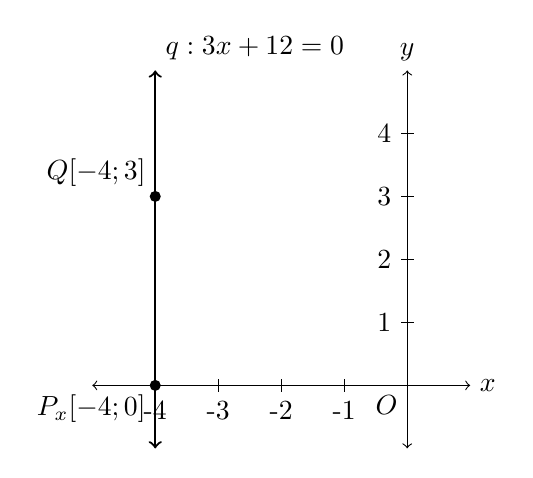
\begin{tikzpicture}[scale=0.8]
            % Osy
            \draw[<->] (-5,0) -- (1,0) node[right] {$x$};
            \draw[<->] (0,-1) -- (0,5) node[above] {$y$};
            \node[below left] at (0,0) {$O$};

            % Přímka
            \draw[thick, <->] (-4,-1) -- (-4,5)
                node[above right] {$q:3x+12=0$};

            % Jednotky na osách
            \foreach \x in {-4,-3,-2,-1} {
                \draw (\x,0.1) -- (\x,-0.1) node[below] {\x};
            }
            \foreach \y in {1,2,3,4} {
                \draw (0.1,\y) -- (-0.1,\y) node[left] {\y};
            }

            % Body
            \fill (-4,0) circle (2.5pt) node[below left] {$P_x[-4;0]$};
            \fill (-4,3) circle (2.5pt) node[above left] {$Q[-4;3]$};
        \end{tikzpicture}
        \caption{Přímka $q:3x+12=0$ je rovnoběžná s osou $y$.}
        \label{fig:Line_parallel_y_axis}
    \end{figure}
\end{example}

\paragraph{Přímka procházející počátkem soustavy souřadnic.}

Jestliže $c=0$, má rovnice tvar
\[
    ax+by=0.
\]
Počátek soustavy souřadnic $O[0;0]$ tuto rovnici vždy splňuje, protože
\[
    a\cdot0+b\cdot0=0.
\]
Každá přímka s nulovým absolutním členem tedy prochází počátkem.

Zvláštními případy jsou také samotné souřadnicové osy:
\[
    x=0
    \qquad\text{je rovnice osy }y,
\]
\[
    y=0
    \qquad\text{je rovnice osy }x.
\]

\begin{example}\label{exa:Special_general_line_equations}
    Určete geometrický význam následujících rovnic:
    \begin{align*}
        p &: 2y-6=0,\\
        q &: 3x+12=0,\\
        r &: 4x-2y=0.
    \end{align*}

    U přímky $p$ je koeficient u $x$ nulový. Po úpravě dostáváme
    \[
        y=3.
    \]
    Jde tedy o vodorovnou přímku rovnoběžnou s osou $x$.

    U přímky $q$ je koeficient u $y$ nulový. Po úpravě dostáváme
    \[
        x=-4.
    \]
    Jde tedy o svislou přímku rovnoběžnou s osou $y$.

    U přímky $r$ je absolutní člen nulový, a proto přímka prochází
    počátkem soustavy souřadnic. Například body
    \[
        O[0;0]
        \qquad\text{a}\qquad
        A[1;2]
    \]
    její rovnici splňují.
\end{example}

\subsubsection{Souhrnný příklad s trojúhelníkem}
\label{subsubsec:General_lines_triangle}

Vrátíme se nyní k trojúhelníku $KLM$ z příkladu~\ref{exa:Parametric_lines_in_triangle}. Tentokrát budeme významné
přímky spojené s trojúhelníkem zapisovat pomocí obecných rovnic.
Příklad tak znovu propojí souřadnice bodů, středy úseček, směrové
a normálové vektory i kolmost přímek.

\begin{example}\label{exa:General_lines_in_triangle}
    Je dán trojúhelník $KLM$ s vrcholy
    \[
        K[-1;4],
        \qquad
        L[5;6],
        \qquad
        M[-3;-2].
    \]
    Trojúhelník je znázorněn na obrázku~\ref{fig:Parametric_lines_in_triangle}.

    Určete obecné rovnice přímek, na nichž leží:
    \begin{enumerate}[label=\alph*)]
        \item strana $LM$,
        \item výška $v_m$ vedená z vrcholu $M$,
        \item osa strany $KL$,
        \item těžnice $t_L$ vedená z vrcholu $L$,
        \item střední příčka spojující středy stran $KL$ a $KM$.
    \end{enumerate}

    Středy stran $KL$ a $KM$ budeme označovat $S_{KL}$ a $S_{KM}$.

    \begin{enumerate}[label=\alph*), leftmargin=2em]

        \item \textbf{Přímka, na níž leží strana $LM$}

        Přímka prochází body $L[5;6]$ a $M[-3;-2]$. Její směrový
        vektor je
        \[
            \overrightarrow{LM}
            =
            (-3-5;-2-6)
            =
            (-8;-8).
        \]

        Použijeme jednodušší směrový vektor
        \[
            \vec{u}_{LM}=(-1;-1).
        \]
        K němu zvolíme normálový vektor
        \[
            \vec{n}_{LM}=(1;-1).
        \]

        Rovnice přímky má tvar
        \[
            x-y+c=0.
        \]
        Dosadíme bod $L[5;6]$:
        \begin{align*}
            5-6+c&=0,\\
            c&=1.
        \end{align*}

        Přímka obsahující stranu $LM$ má rovnici
        \[
            p_{LM}: x-y+1=0.
        \]

        Ověření bodem $M[-3;-2]$:
        \[
            -3-(-2)+1=0.
        \]

        \item \textbf{Výška $v_m$ vedená z vrcholu $M$}

        Výška $v_m$ je kolmá ke straně $KL$. Směrový vektor strany
        $KL$ je
        \[
            \overrightarrow{KL}
            =
            (5-(-1);6-4)
            =
            (6;2).
        \]
        Použijeme jednodušší vektor
        \[
            \vec{u}_{KL}=(3;1).
        \]

        Protože je výška $v_m$ ke straně $KL$ kolmá, může být vektor
        $\vec{u}_{KL}$ normálovým vektorem výšky:
        \[
            \vec{n}_{v_m}=(3;1).
        \]

        Rovnice výšky má tvar
        \[
            3x+y+c=0.
        \]
        Dosadíme vrchol $M[-3;-2]$:
        \begin{align*}
            3\cdot(-3)+(-2)+c&=0,\\
            -11+c&=0,\\
            c&=11.
        \end{align*}

        Výška $v_m$ má rovnici
        \[
            v_m: 3x+y+11=0.
        \]

        \item \textbf{Osa strany $KL$}

        Osa strany $KL$ prochází jejím středem a je ke straně $KL$
        kolmá. Nejprve určíme střed strany:
        \begin{align*}
            S_{KL}
            &=
            \left[
                \frac{-1+5}{2};
                \frac{4+6}{2}
            \right] = [2;5].
        \end{align*}

        Osa strany $KL$ je stejně jako výška $v_m$ kolmá ke straně
        $KL$, a proto můžeme použít stejný normálový vektor
        \[
            \vec{n}_{o_{KL}}=(3;1).
        \]

        Rovnice osy má tvar
        \[
            3x+y+c=0.
        \]
        Dosadíme bod $S_{KL}[2;5]$:
        \begin{align*}
            3\cdot2+5+c&=0,\\
            11+c&=0,\\
            c&=-11.
        \end{align*}

        Osa strany $KL$ má rovnici
        \[
            o_{KL}: 3x+y-11=0.
        \]

        Výška $v_m$ a osa strany $KL$ mají rovnoběžné normálové
        vektory, ale různé absolutní členy. Jsou tedy navzájem
        rovnoběžné.

        \item \textbf{Těžnice $t_L$ vedená z vrcholu $L$}

        Těžnice $t_L$ spojuje vrchol $L$ se středem protější strany
        $KM$. Nejprve určíme tento střed:
        \begin{align*}
            S_{KM}
            &=
            \left[
                \frac{-1+(-3)}{2};
                \frac{4+(-2)}{2}
            \right] = [-2;1].
        \end{align*}

        Směrový vektor těžnice je
        \[
            \overrightarrow{LS_{KM}}
            =
            (-2-5;1-6)
            =
            (-7;-5).
        \]
        K tomuto směrovému vektoru zvolíme normálový vektor
        \[
            \vec{n}_{t_L}=(5;-7),
        \]
        protože
        \[
            (-7;-5)\cdot(5;-7)=-35+35=0.
        \]

        Rovnice těžnice má tvar
        \[
            5x-7y+c=0.
        \]
        Dosadíme vrchol $L[5;6]$:
        \begin{align*}
            5\cdot5-7\cdot6+c&=0,\\
            25-42+c&=0,\\
            c&=17.
        \end{align*}

        Těžnice $t_L$ má rovnici
        \[
            t_L: 5x-7y+17=0.
        \]

        \item \textbf{Střední příčka $S_{KL}S_{KM}$}

        Již známe oba středy:
        \[
            S_{KL}[2;5],
            \qquad
            S_{KM}[-2;1].
        \]

        Směrový vektor střední příčky je
        \[
            \overrightarrow{S_{KL}S_{KM}}
            =
            (-2-2;1-5)
            =
            (-4;-4).
        \]
        Použijeme jednodušší směrový vektor
        \[
            \vec{u}_s=(-1;-1)
        \]
        a k němu normálový vektor
        \[
            \vec{n}_s=(1;-1).
        \]

        Rovnice přímky obsahující střední příčku má tvar
        \[
            x-y+c=0.
        \]
        Dosadíme bod $S_{KL}[2;5]$:
        \begin{align*}
            2-5+c&=0,\\
            c&=3.
        \end{align*}

        Přímka obsahující střední příčku má rovnici
        \[
            s: x-y+3=0.
        \]

        Přímky
        \[
            p_{LM}:x-y+1=0
        \]
        a
        \[
            s:x-y+3=0
        \]
        mají stejné koeficienty u proměnných $x$ a $y$, ale různé
        absolutní členy. Jsou tedy rovnoběžné, čímž se opět potvrzuje známá
        vlastnost střední příčky trojúhelníku:
        \[
            S_{KL}S_{KM}\parallel LM.
        \]

    \end{enumerate}
\end{example}

\begin{example}\label{exa:Central_symmetry_line}
    Je dána přímka
    \[
        p:2x-y+1=0.
    \]
    Určete rovnici přímky $p'$, která je obrazem přímky $p$ ve
    středové souměrnosti se středem
    \[
        S[-2;1].
    \]

    Situace je znázorněnáo na obrázku \ref{fig:Central_symmetry_line}.
    
    Přímku $p'$ můžeme určit pomocí obrazů dvou různých bodů přímky
    $p$. Pro obraz libovolného bodu $X$ ve středové souměrnosti se
    středem $S$ platí
    \[
        X'=S+(S-X)=2S-X.
    \]

    Nejprve tedy na přímce $p$ zvolíme dva různé body, určíme jejich
    obrazy a následně sestavíme rovnici přímky procházející těmito
    obrazy.

    Zvolíme nejprve bod s první souřadnicí $x=0$. Dosadíme do rovnice
    přímky $p$:
    \begin{align*}
        2\cdot0-y+1&=0,\\
        -y+1&=0,\\
        y&=1.
    \end{align*}

    Na přímce $p$ tedy leží bod
    \[
        A[0;1].
    \]

    Jako druhý bod zvolíme bod s první souřadnicí $x=1$:
    \begin{align*}
        2\cdot1-y+1&=0,\\
        3-y&=0,\\
        y&=3.
    \end{align*}

    Druhým bodem přímky $p$ je
    \[
        B[1;3].
    \]

    Nyní určíme obraz bodu $A$ ve středové souměrnosti se středem
    $S[-2;1]$:
    \begin{align*}
        A'
        &=
        S+(S-A)\\
        &=
        [-2;1]+\bigl([-2;1]-[0;1]\bigr)\\
        &=
        [-2;1]+(-2;0)\\
        &=
        [-4;1].
    \end{align*}

    Obdobně určíme obraz bodu $B$:
    \begin{align*}
        B'
        &=
        S+(S-B)\\
        &=
        [-2;1]+\bigl([-2;1]-[1;3]\bigr)\\
        &=
        [-2;1]+(-3;-2)\\
        &=
        [-5;-1].
    \end{align*}

    Obrazem přímky $p$ je přímka $p'$, která prochází body
    \[
        A'[-4;1]
        \qquad\text{a}\qquad
        B'[-5;-1].
    \]

    Její směrový vektor můžeme určit jako
    \[
        \overrightarrow{A'B'}
        =
        (-5-(-4);-1-1)
        =
        (-1;-2).
    \]

    K tomuto směrovému vektoru zvolíme normálový vektor
    \[
        \vec{n}_{p'}=(2;-1),
    \]
    protože
    \[
        (-1;-2)\cdot(2;-1)
        =
        -2+2
        =
        0.
    \]

    Obecná rovnice přímky $p'$ má tedy tvar
    \[
        2x-y+c=0.
    \]

    Dosadíme například bod $A'[-4;1]$:
    \begin{align*}
        2\cdot(-4)-1+c&=0,\\
        -8-1+c&=0,\\
        c&=9.
    \end{align*}

    Hledaná přímka má rovnici
    \[
        p':2x-y+9=0.
    \]

    Přímky $p$ a $p'$ mají stejné normálové vektory, a jsou proto
    rovnoběžné. To odpovídá vlastnosti středové souměrnosti: obrazem
    přímky, která neprochází středem souměrnosti, je přímka s ní
    rovnoběžná.

    \begin{figure}[H]
        \centering
        \begin{tikzpicture}[scale=0.9]

            % Přímky
            \draw[thin, <->]
                (-1.5,-2) -- (2.5,6)
                node[above right] {$p$};

            \draw[thin, <->]
                (-5.5,-2) -- (-1.5,6)
                node[above right] {$p'$};

            % Body
            \coordinate (A) at (0,1);
            \coordinate (B) at (1,3);
            \coordinate (S) at (-2,1);
            \coordinate (Ap) at (-4,1);
            \coordinate (Bp) at (-5,-1);

            \fill (A) circle (2.5pt)
                node[below right] {$A$};
            \fill (B) circle (2.5pt)
                node[below right] {$B$};
            \fill (S) circle (2.5pt)
                node[above right] {$S$};
            \fill (Ap) circle (2.5pt)
                node[above left] {$A'$};
            \fill (Bp) circle (2.5pt)
                node[below left] {$B'$};

            % Spojnice bodů se středem
            \draw[vector] (A) -- (S);
            \draw[vector] (S) -- (Ap);

            \draw[vector] (B) -- (S);
            \draw[vector] (S) -- (Bp);

        \end{tikzpicture}
        \caption{Přímka $p'$ je obrazem přímky $p$ ve středové
        souměrnosti se středem $S$.}
        \label{fig:Central_symmetry_line}
    \end{figure}
\end{example}